% This is samplepaper.tex, a sample chapter demonstrating the
% LLNCS macro package for Springer Computer Science proceedings;
% Version 2.20 of 2017/10/04
%
\documentclass[runningheads]{llncs}
%
\usepackage{graphicx}
\usepackage{hyperref}
\usepackage{amsmath}

% Used for displaying a sample figure. If possible, figure files should
% be included in EPS format.
%
% If you use the hyperref package, please uncomment the following line
% to display URLs in blue roman font according to Springer's eBook style:
% \renewcommand\UrlFont{\color{blue}\rmfamily}

%\usepackage[utf8x]{inputenc}
%\usepackage[english,russian]{babel}


\begin{document}
%
\title{Acceleration of Global Search by Implementing Dual Estimates for Lipschitz Constant\thanks{This research was supported by the the Russian Science Foundation, project No.\,16-11-10150.}}
%
\titlerunning{Acceleration of Global Search}
% If the paper title is too long for the running head, you can set
% an abbreviated paper title here
%
\author{Roman Strongin%\orcidID{0000-0003-0390-6695} 
\and Konstantin Barkalov%\orcidID{0000-0001-5273-2471} 
\and Semen Bevzuk%\orcidID{0000-0002-3845-5356}
}
%
\authorrunning{R. Strongin et al.}
% First names are abbreviated in the running head.
% If there are more than two authors, 'et al.' is used.
%
\institute{
Lobachevsky State University of Nizhni Novgorod, Nizhni Novgorod, Russia
\email{konstantin.barkalov@itmm.unn.ru}
}
%
\maketitle              % typeset the header of the contribution
%
\begin{abstract}
The paper considers global optimization problems with a black-box objective 
function satisfying the Lipschitz condition. Efficient algorithms for this 
class of problems require reliable estimates of the Lipschitz constant to be 
introduced. The various approaches have been proposed to take into account both
global and local properties of the objective function. In particular, algorithms
using local estimates of the Lipschitz constant have shown their potential.
The new approach presented in this paper is based on simultaneous use of two
estimates: one is substantially larger than the other. 
The larger estimate ensures global convergence and the smaller one reduces 
the total number of trials needed to find the global optimizer.
Results of numerical experiments on the random sample of multidimensional 
functions demonstrate the efficiency of the suggested approach.  

\keywords{Global optimization \and Multiextremal problems 
\and Lipschitz constant estimates}
\end{abstract}
%
%
%
\section{Introduction}

The paper considers global optimization problems of the form 
\begin{gather}
 \varphi(y^\ast)=\min{\left\{\varphi(y):y\in D\right\}}, \label{problem}\\
 D=\left\{y\in R^N: a_i\leq y_i \leq b_i, 1\leq i \leq N\right\} \label{D},
\end{gather}
where the objective function is a black-box function and assumed to satisfy the Lipschitz condition
\[
\left|\varphi(y_1)-\varphi(y_2)\right|\leq L\left\|y_1-y_2\right\|,\; y_1,y_2 \in D,
\]
with the constant $L$ unknown a priori.

%Russian
The assumption of the objective function to be Lipschitzian is typical for many approaches to the development of the global optimization algorithms \cite{Evtushenko2013,Zilinskas2010,Pinter1996,Strongin2000}. At that, the adaptive estimate of the unknown Lipschitz constant based on the obtained search information is the most important problem being solved in these algorithms anyway. 
The Lipschitz constant value affects the convergence rate of the global optimization algorithms essentially. Therefore, the issue of its correct estimate is so important. 
The underestimate of the constant true value may result in losing the convergence of the algorithm to the global solution. At the same time, too large value of the estimate of the constant for the objective function not matching its real behavior results in slow convergence of the algorithm to the global minimizer. 

Several typical methods of adaptive estimation of the Lipschitz constant are known:
\begin{itemize}
	\item global estimation of the constant $L$ in the whole search domain $D$ \cite{Horst1996,Pinter1996,Strongin2000}.
	\item local estimations of the constants $L_i$ in different subdomains $D_i$ of the search domain $D$ \cite{Kvasov2003,Sergeyev2010,Sergeyev2016}.
	\item the choice of the estimates of the constant $L$ from a set of possible values \cite{Gablonsky2001,Jones1993,Jones2009,Sergeyev2006}.
\end{itemize}

Each approach from the above has its own advantages and disadvantages. For example, the use of the global estimate over the whole search domain can slow down the convergence of the algorithm to the global minimizer. The use of the local estimates accelerating the convergence requires an adequate adjustment of the algorithm parameters in order to preserve the global convergence. 

In the present work, an algorithm, in which it is proposed to use two global estimates of the Lipschitz constant, one being much greater than another, is considered. 
The larger estimate ensures global convergence and the smaller one reduces the total number of trials needed to find the global optimizer.
The choice of the one of two estimates to be used in the algorithm rules is performed adaptively subject to the function behavior and to the search phase.

The rigorous substantiation of the proposed approach goes beyond the present initial publication and will be done in the forthcoming works. Here we present the results of numerical experiments clearly demonstrating the efficiency of the novel algorithm. When conducting the numerical experiments, several hundred multiextremal test problems of various dimensionalities have been solved.

\section{Global search algorithm and dimensionality reduction}
%Russian 

The adaptation of the efficient algorithms of solving the one-dimensional problems to solving the multidimensional problems is typical method of constructing the global optimization algorithms, see, for example, the diagonal partitions method in \cite{Sergeyev2006} or the simplicial partitions method in \cite{Zilinskas2008}.

In the present paper, the approach based on the ideas of dimensionality reduction with the use of the Peano-Hilbert curves \cite{Sergeyev2013,Strongin2000}, which continuously and unambiguously maps the unit interval $[0,1]$ onto the $n$-dimensional cube $D$ from (\ref{D}) has been used. By using this kind of mapping, it is possible to reduce the multidimensional problem (\ref{problem}) to a univariate problem
\[
\varphi(y^\ast)=\varphi(y(x^\ast))=\min{\left\{\varphi(y(x)): x\in[0,1]\right\}},
\]
where the function $\varphi(y(x))$ will satisfy a uniform H{\"o}lder condition
\[
\left|\varphi(y(x_1))-\varphi(y(x_2))\right|\leq H\left|x_1-x_2\right|^{1/N},
\]
with the H{\"o}lder constant $H$ linked to the Lipschitz constant $L$ by the relation
$ H=2 L \sqrt{N+3}$.

Let us call the process of computing a function value (including the construction of the image $y=y(x)$) a \textit{trial}, and the pair $\{x, z = \varphi(y(x))\}$ the outcome of the trial.

The global search algorithm (according to \cite{Strongin2000}) can be formulated as follows.
The first two trials are executed at 
the points $y^0=y(0), y^1=y(1)$. The choice of the point $y^{k+1},k\geq 1,$  
for the next $(k+1)^{\rm th}$ trial is defined by the following rules.

\begin{enumerate}
	\item 
	Renumber the preimages of all the points $y^i=y(x^i)$
	from the trials already performed  	
%\begin{equation}\label{y_i} 
%y^0=y(x^0), y^1=y(x^1),...,y^k=y(x^k)
%\end{equation}
by subscripts in the increasing order of their coordinates, i.e.
\begin{equation}\label{x_i}
0=x_0<x_1<\dots <x_k=1,
\end{equation}
and associate these with the values $z_i=\varphi(y(x_i)), 0\leq i \leq k,$ 
computed at these points.
\item
Compute the maximum absolute value of the first divided differences
\begin{equation}\label{mu}
\mu = \max_{1 \leq i \leq k}\frac{\left|z_i-z_{i-1}\right|}{\Delta_i},
\end{equation}
where $\Delta_i=\left(x_i-x_{i-1}\right)^{1/N}$. If $\mu = 0$, set $\mu = 1$.
\item
For each interval $(x_{i-1}, x_i), \; 1\leq i \leq k,$  calculate the value 
$R(i)$ called the \textit{characteristic} of the interval
\begin{equation}\label{R}
R(i)=\Delta_i+\frac{(z_i-z_{i-1})^2}{r^2\mu^2\Delta_i}-2\frac{z_i+z_{i-1}-2z^*}{r\mu},
\end{equation}
where 
\begin{equation}\label{z}
z^*= \min_{0\leq i\leq k}z_i
\end{equation} 
and the real number $r>1$ is 
the input parameter of the algorithm.
\item 
Select the interval $(x_{t-1},x_t)$ corresponding to the maximum characteristic
\begin{equation}\label{MaxR}
R(t)= \max_{1 \leq i \leq k}R(i).
\end{equation}
\item
Carry out the next trial at the point $x^{k+1}\in(x_{t-1},x_t)$ calculated using
the following formula
\begin{equation}\label{xk1}
x^{k+1} = \frac{x_t+x_{t-1}}{2} - \mathrm{sign}(z_t-z_{t-1})\frac{1}{2r}
\left[\frac{\left|z_t-z_{t-1}\right|}{\mu}\right]^N.
\end{equation}
\end{enumerate}

The algorithm terminates if the condition $\Delta_t < \epsilon$ is satisfied
where $t$ is from (\ref{MaxR}), and $\epsilon>0$ is the predefined accuracy. 

The theory of convergence of this algorithm is provided in \cite{Strongin2000}. 
The algorithm is allows for an efficient
parallelization for shared and distributed memory \cite{Gergel2003}  and for accelerators \cite{Gergel2016}.


\section{Algorithm with Dual Lipschitz Constant Estimates}

%Russian
The global search algorithm presented in previous section is intended for solving the multiextremal problems, in which the objective function satisfies the Lipschitz condition. It is not necessary to define the value of the constant for the algorithm convergence. The estimation of the constant is performed in the course of global search on the base of available search information. 
According to the theorem from \cite{Strongin2000}, the sequence of the trial points $\{y^k\}$ will converge to the global minimizer $y^*$ if the condition 
\begin{equation}\label{cond}
r\mu > 2^{3-1/N}L\sqrt{N+3}.
\end{equation}
\noindent is satisfied. Thus,  an appropriate choice of the parameter $r$ from (\ref{R}) allows using the value $r\mu / 2^{3-1/N}\sqrt{N+3}$ as an estimate of the Lipschitz constant for the objective function $\varphi(y)$.

Satisfying the condition (\ref{cond}) will be guaranteed at choosing large enough value of the parameter $r$. However, in this case the method will perform a large number of trials until the stop condition is satisfied.
The choice of small value of the parameter $r$ (that corresponds to the lower estimate of the Lipschitz constant) would considerably reduce the number of trials but may violate the convergence to the global extremum.

An approach, in which two estimates of the Lipschitz constant %, one of which is essentially greater than another, 
are used in the rules of algorithm, is a promising one. 
This approach implies the use of two parameters $r_{glob}$ and $r_{loc}$ where $r_{glob} > r_{loc}$ in the algorithm.

The rules of the algorithm with two estimates of the Lipschitz constant reproduce the ones of global search algorithm completely except Rule 3 (computing the characteristic).

New rule of calculating the characteristic $R(i)$ of the interval $(x_{i-1}, x_i)$ will consist of the following operations:
\begin{itemize}
\item
Calculate the value $R_{glob}(i)$ corresponding to the larger estimate of the Lipschitz constant
\[
R_{glob}(i)=\Delta_i+\frac{(z_i-z_{i-1})^2}{r_{glob}^2\mu^2\Delta_i}-2\frac{z_i+z_{i-1}-2z^*}{r_{glob}\mu}.
\]
\item
Calculate the value $R_{loc}(i)$ corresponding to the smaller estimate of the Lipschitz constant
\[
R_{loc}(i)=\Delta_i+\frac{(z_i-z_{i-1})^2}{r_{loc}^2\mu^2\Delta_i}-2\frac{z_i+z_{i-1}-2z^*}{r_{loc}\mu}.
\]
\item
Determine the characteristic $R(i)$ as
\begin{equation}\label{pho}
R(i) = \max\{\rho R_{loc}(i),R_{glob}(i)\}, \textrm{where} \; \rho = \left(\frac{1-1/r_{glob}}{1-1/r_{loc}}\right)^2,
\end{equation}
and fix the value $r = r_{loc}$ if $\rho R_{loc}(i) > R_{glob}(i)$, otherwise fix $r=r_{glob}$.
\item
This value of $r$ is used in Rule 5 of the algorithm in the computing of the next trial point.   
\end{itemize}.

This method of computing the characteristic is substantiated as follows. 
Let current minimum value of $z^*$ from (\ref{z}) is achieved at the left point of the $i^{\rm th}$ interval, i.e. $z^* = z_{i-1}$. Then, according to the rule (\ref{R}) the following inequality will be true: 
\[
R(i) \geq \Delta_i \left( 1 - \frac{1}{r} \right)^2.
\]
Consequently, two lower estimates of the two characteristics of current best interval $R_{loc}(i)$ and $R_{glob}(i)$ calculated with different parameters $r_{loc}$ and $r_{glob}$ will take different values.
However, if the former is multiplied by the coefficient $\rho$ from (\ref{pho}), the lower estimates of the characteristics of the best interval would match each other that would make the characteristics calculated for other intervals comparable as well.

\section{Numerical Experiments}

The numerical comparison of the algorithms has been carried out using the GKLS 
test problem generator \cite{Gaviano2003}. 
This generator of multiextremal functions is often used for the investigations of the global 
optimization algorithms ~\cite{Barkalov2018,Paulavicius2014,Sergeyev2015}.
Six GKLS classes of differentiable test functions of the dimensions $N = 3,4,5$
have been used. For each dimension, both \textit{Hard} and \textit{Simple}
classes have been considered. The difficulty of a class was increased either by
decreasing the radius of the attraction region of the global minimizer, or by
decreasing the distance from the global minimizer $y^\ast$ to the domain
boundaries. The global minimizer $y^\ast$ was considered to be found, if the
algorithm generated a trial point $y^k$ in the vicinity of the global minimum,
i.e. $\left|y^k-y^\ast\right| <\delta\left\|b-a\right\|$, 
$a$ and $b$ are the boundaries of the search domain $D$. 

%Russian
Each series of problems has been solved by the original global search algorithm (GSA) and by the method with two estimates of the Lipschitz constant (GSA-DL). The evolvent constructed using the parameter $m = 10$ was used for the dimensionality reduction in both algorithms. The relative accuracy of the solution search was $\delta = 0.01$.% for $N=3,4$ and $\delta = 0.02$ for $N=5$. 
The maximum allowable number of iterations per problem was $K_{max} = 10^6$.

The averaged numbers of iterations performed by the algorithms are presented in Table \ref{tab:1}.
At that, for GSA the values of parameter $r=4.8$ when solving the problems of Simple class and $r=5.6$ when solving the problems of Hard class were used. 
These values are the minimum ones (with the accuracy 0.1), at which all problems have been solved successfully.
When solving the problems from the above classes by GSA-DL, the value of parameter $r$ specified above was selected for the upper estimate of the Lipschitz constant, i.e. the value $r_{glob} = r$ was set, which was complemented by the values $r_{loc}=1.8$, $r_{loc}=2.1$ and $r_{loc}=2.4$. 
The number of unsolved problems is specified in brackets.

\begin{table}
	\caption{Average number of iterations}
	\label{tab:1}
	\center
	\begin{tabular}{ccccccccc}
		\hline\noalign{\smallskip}
		 & \multicolumn{2}{c}{$N=3$} & & \multicolumn{2}{c}{$N=4$} & & \multicolumn{2}{c}{$N=5$}  \\
		\noalign{\smallskip} \cline{2-3} \cline{5-6} \cline{8-9} \noalign{\smallskip}
		 & \textit{Simple} & \textit{Hard} & & \textit{Simple} & \textit{Hard} & & \textit{Simple} & \textit{Hard}  \\
		\noalign{\smallskip} \hline \noalign{\smallskip}
									AGS	&	2444	&	5345	& &	28415	&	77470	& & 25220(1) & 126138(4)		\\
AGS-DL, $r_{loc}=1.8$	&	1372	&	2632	& &	13273	&	37715	& &	12702    & 94296(1)			\\
AGS-DL, $r_{loc}=2.1$	&	1502	&	2805	& &	14826	&	38843	& &	15213    & 90792(2)			\\
AGS-DL, $r_{loc}=2.4$	&	1567	&	2868	& &	19447	&	40342	& &	18239    & 106438(2)		\\
		\noalign{\smallskip}\hline
	\end{tabular}
\end{table}


The advantage of the GSA-DL algorithm over its prototype is confirmed by the operational characteristics of the algorithms as well. 

Assume a series of test problems to be solved. The results of solving the series can be presented by a function $p(k)$ featuring the fraction of the total number of problems solved in $k$ iterations. Such a function will be called the \textit{operational characteristic} of the algorithm. 


The operational characteristics for the GSA and GSA-DL methods obtained when solving the \textit{Simple} and \textit{Hard} problem series with the dimensionalities $N=4$ and $N=5$ are presented in Fig. \ref{oper4} and \ref{oper5}, respectively. The values of the parameters $r$ used for estimating the Lipschitz constant are given in the figures.

\begin{figure}
\begin{minipage}{0.5\linewidth}
\center{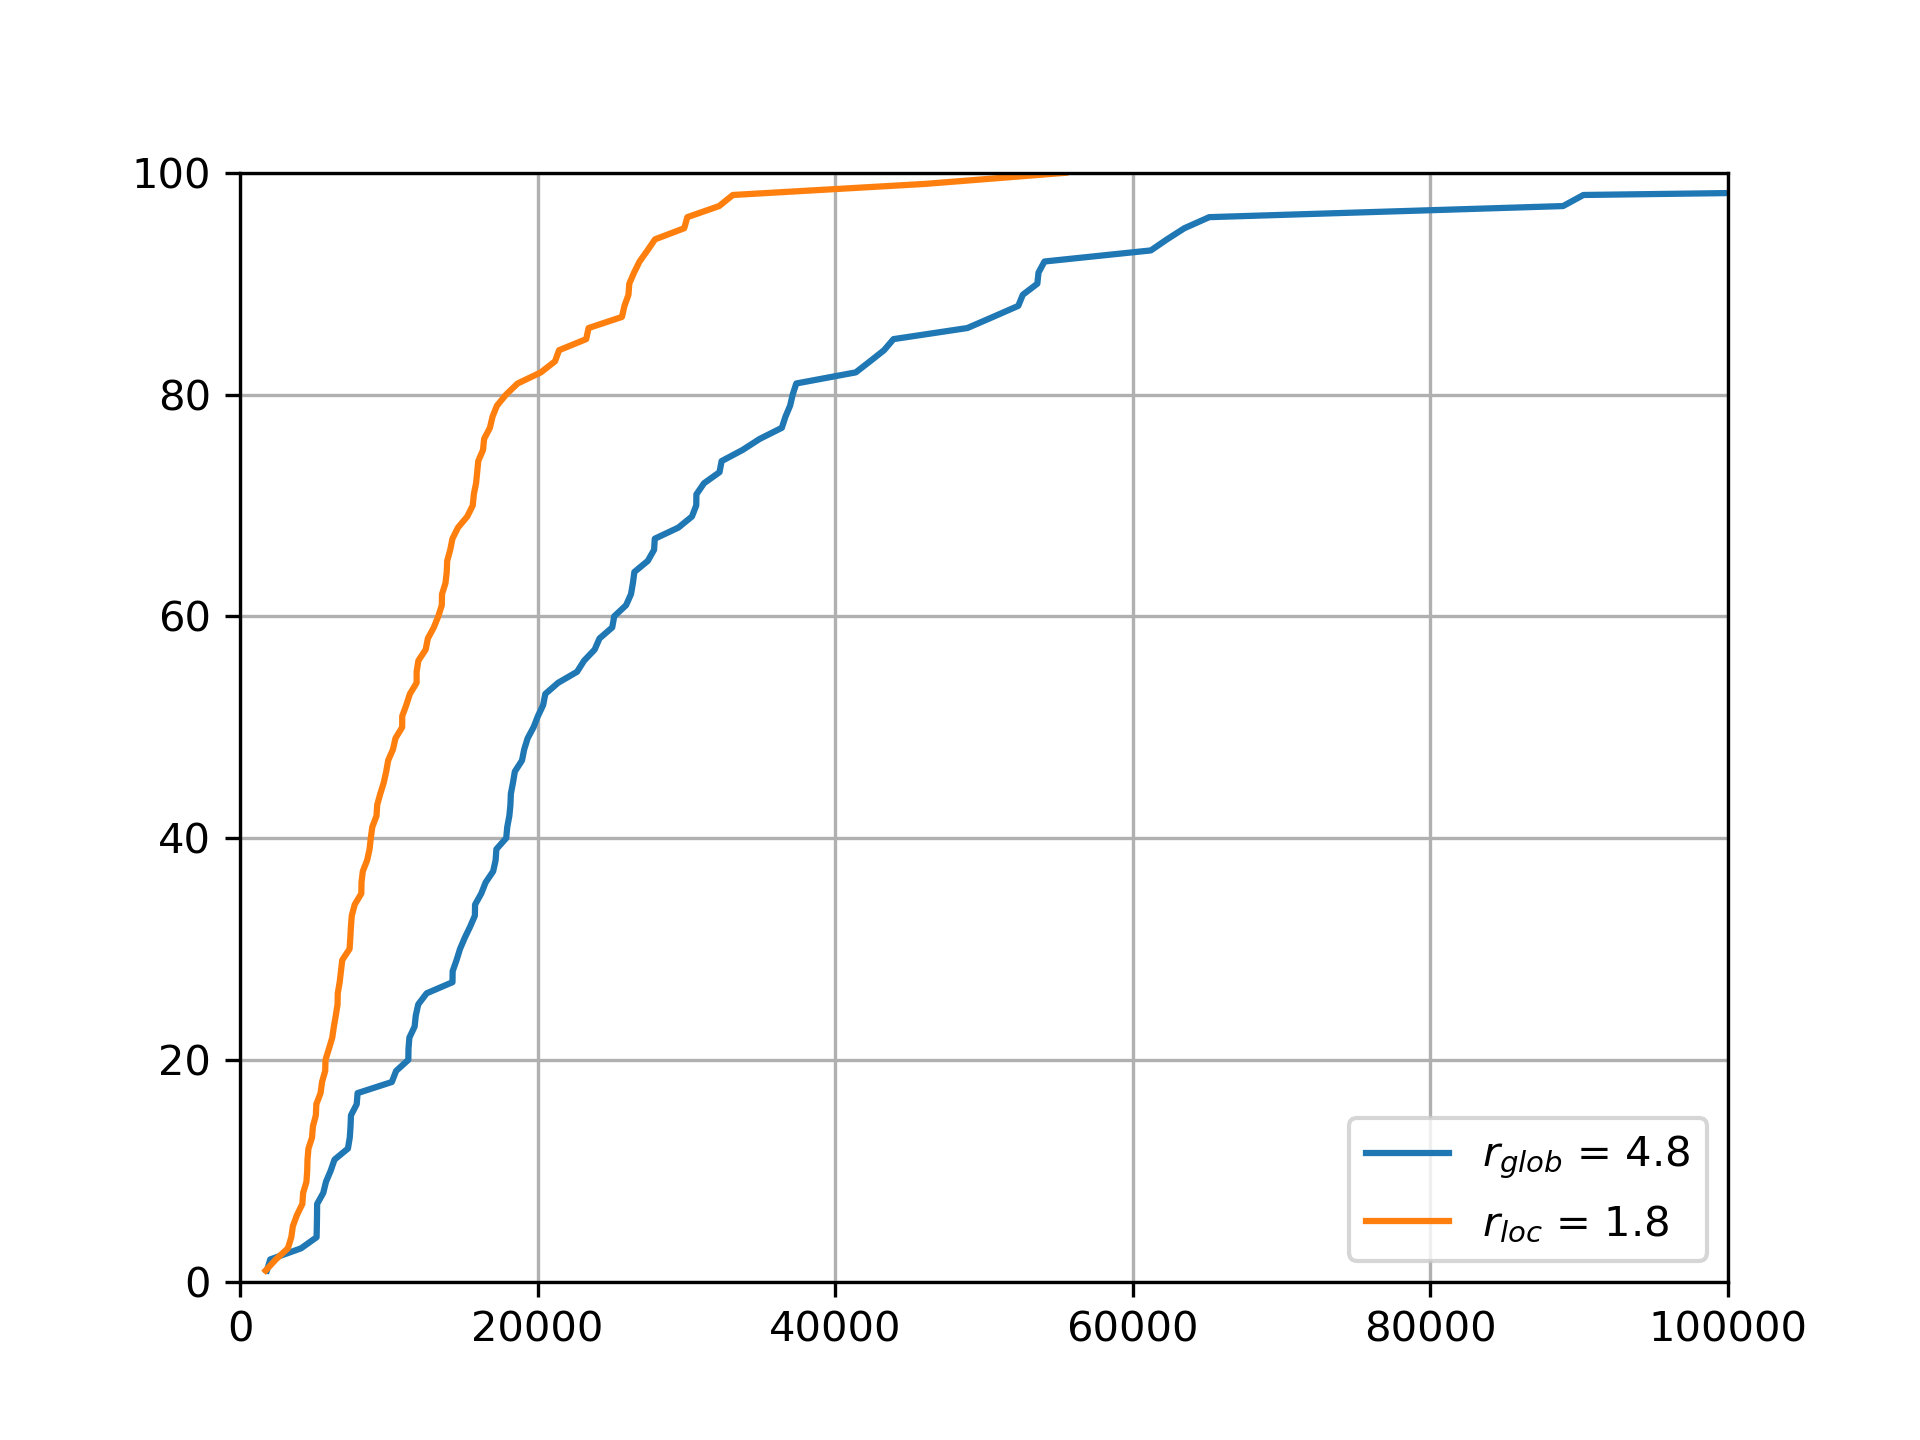
\includegraphics[width=1.0\linewidth]{Operating_characteristic_gklss_4.png} \\ (a)}
\end{minipage}
\hfill
\begin{minipage}{0.5\linewidth}
\center{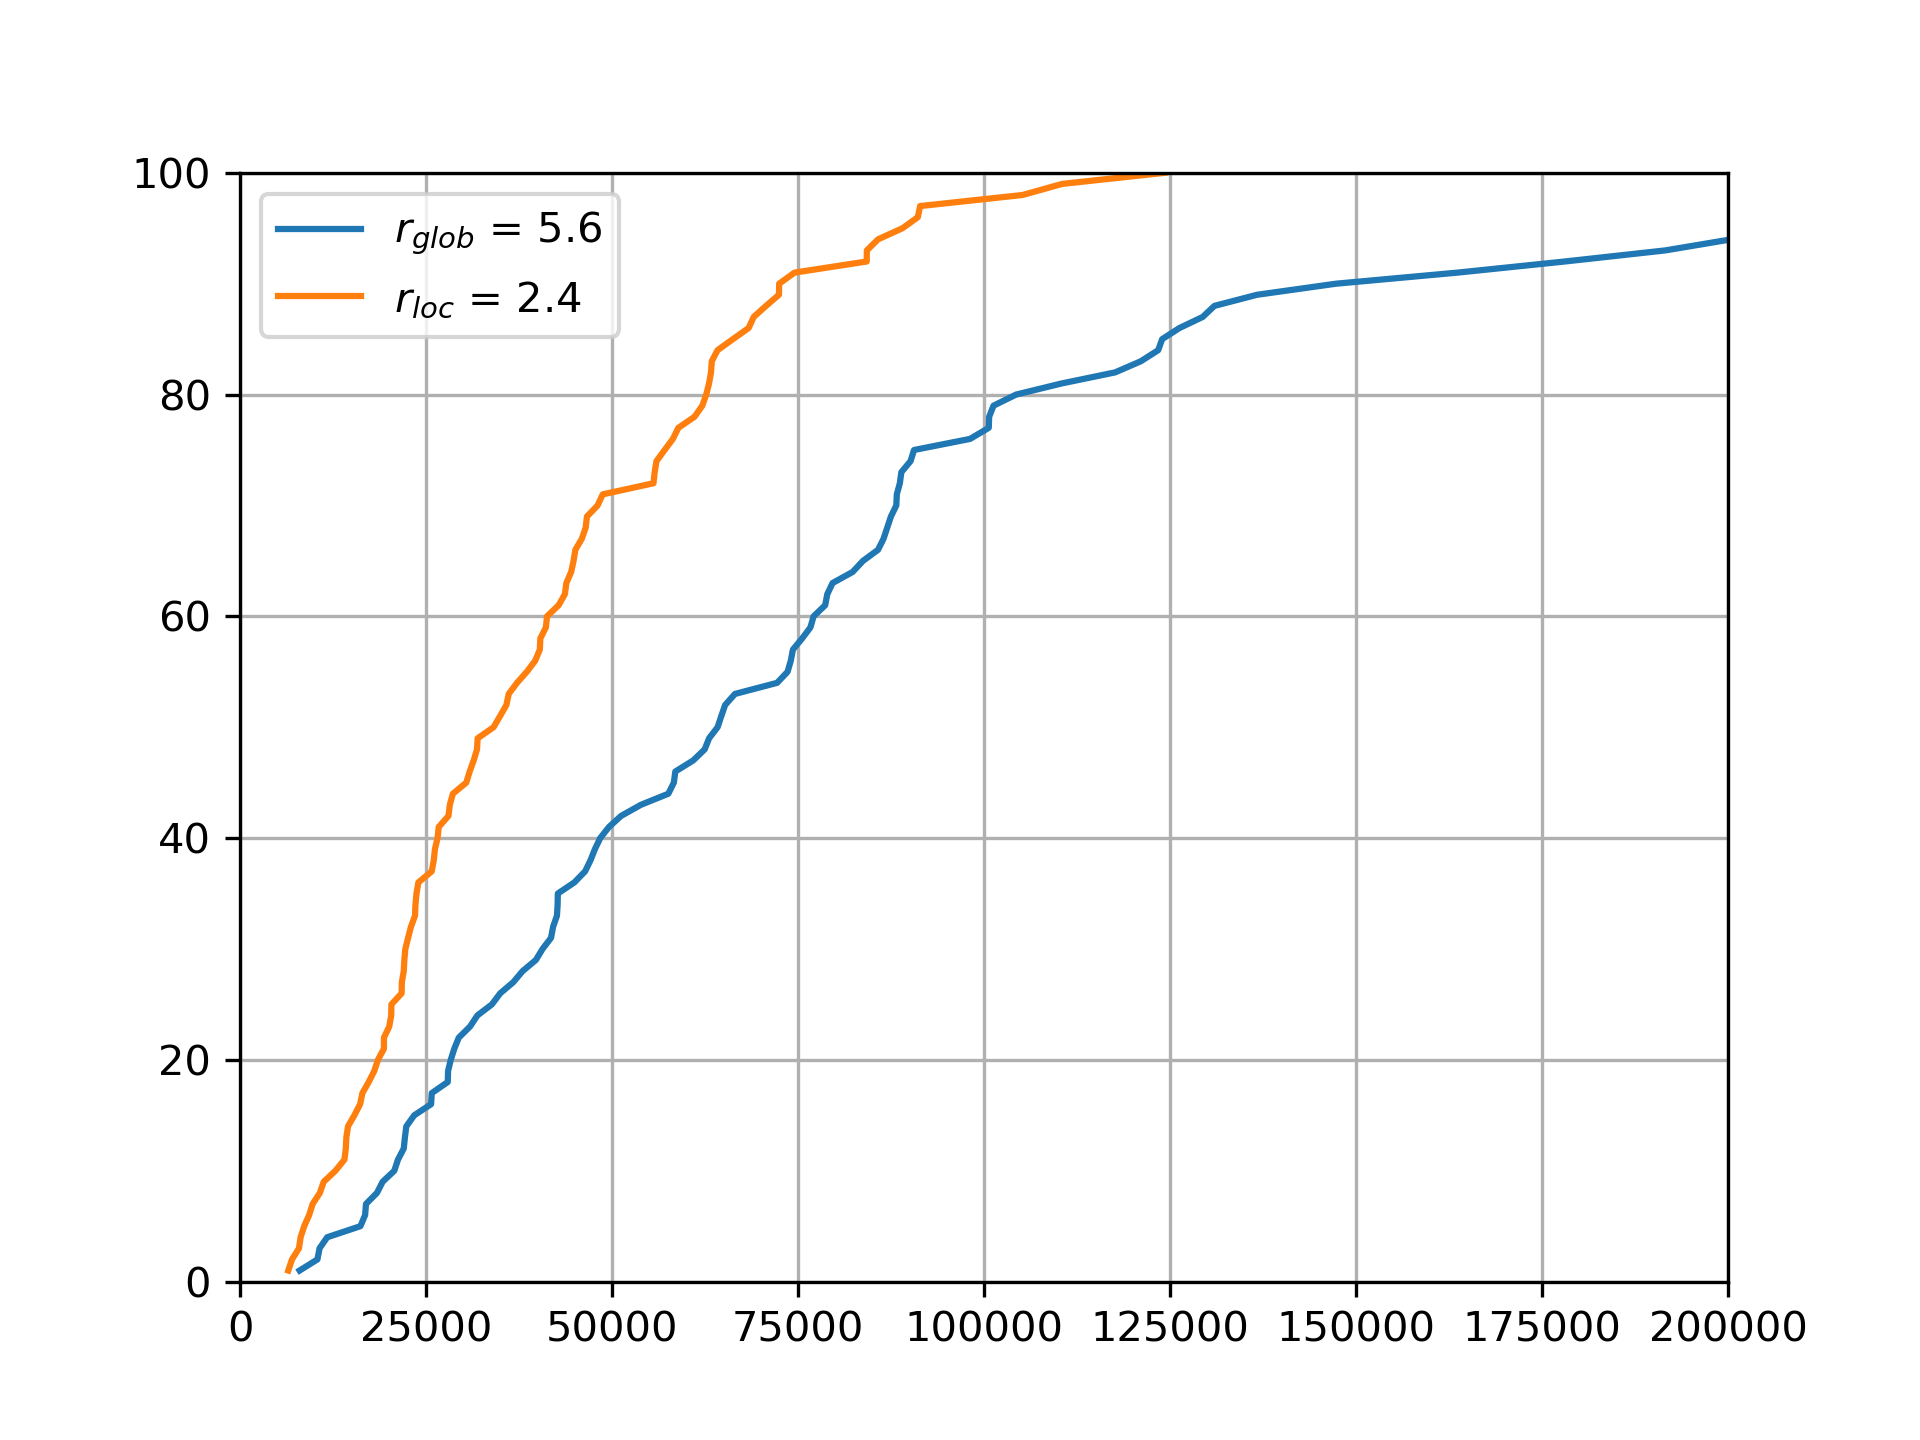
\includegraphics[width=1.0\linewidth]{Operating_characteristic_gklsh_4.png} \\ (b)}
\end{minipage}
\caption{Operational characteristics for GKLS Simple (a) and Hard (b) classes, $N=4$.}
\label{oper4}
\end{figure}

\begin{figure}
\begin{minipage}{0.5\linewidth}
\center{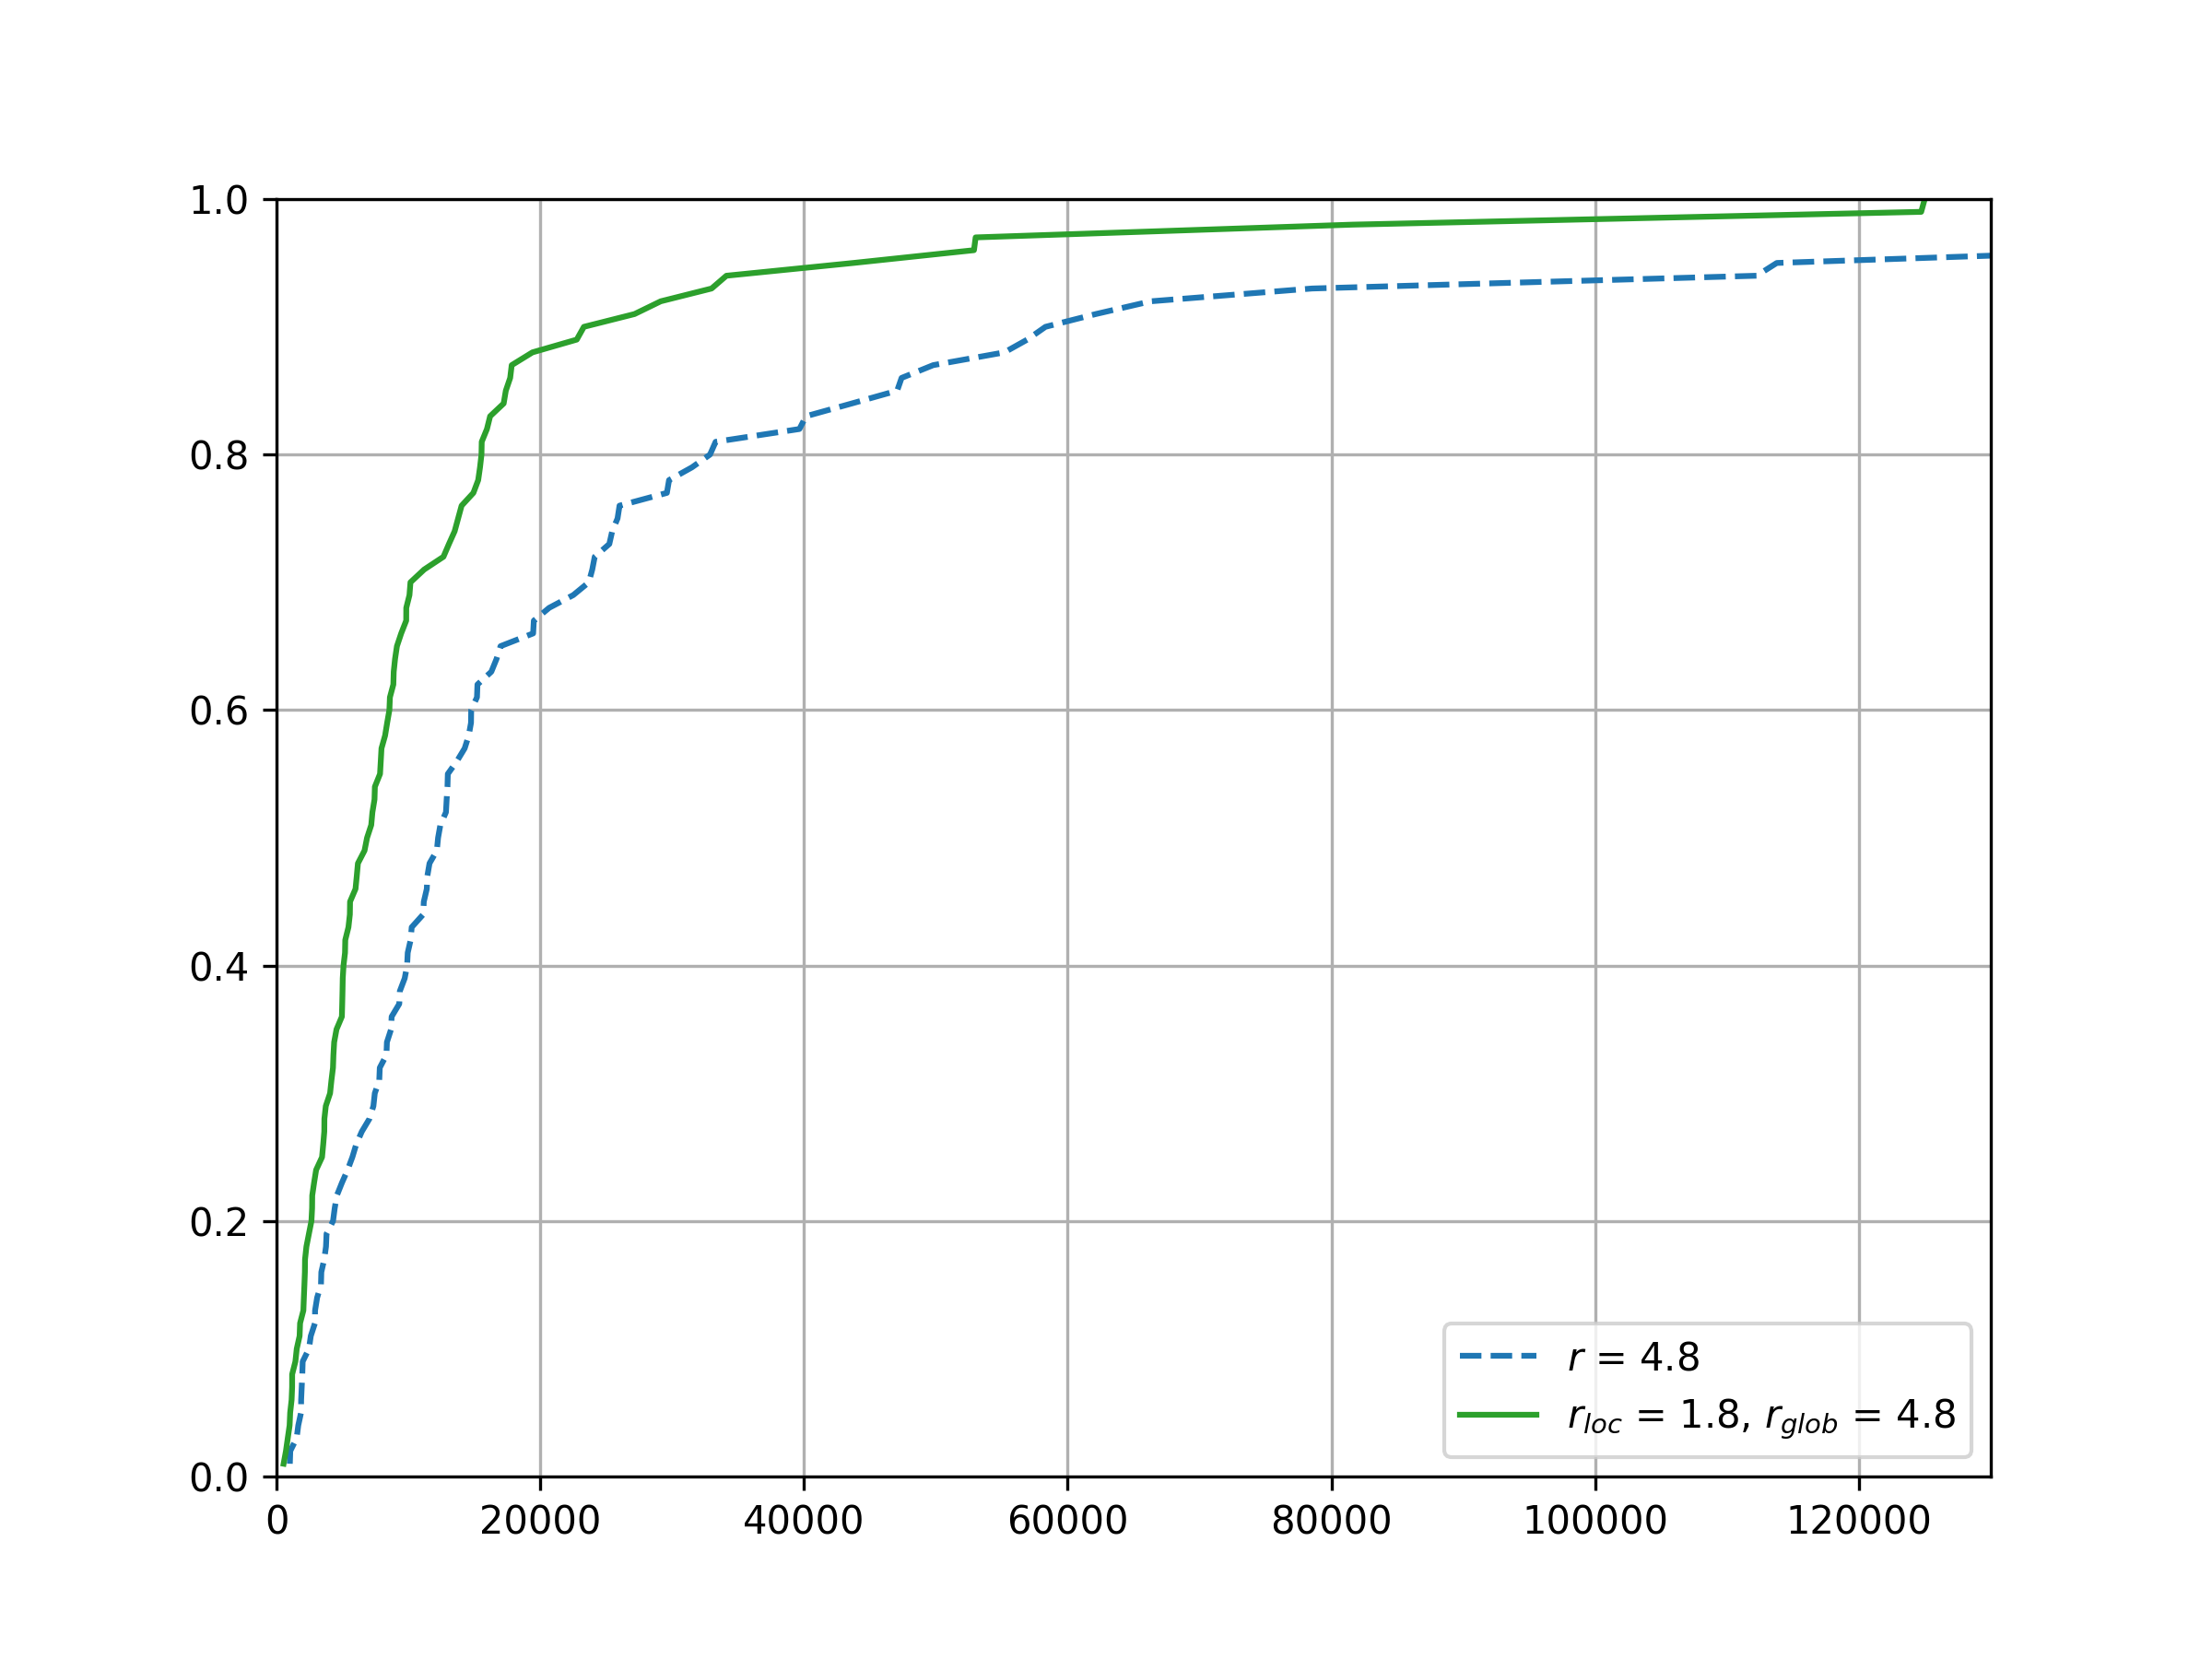
\includegraphics[width=1.0\linewidth]{Operating_characteristic_gklss_5.png} \\ (a)}
\end{minipage}
\hfill
\begin{minipage}{0.5\linewidth}
\center{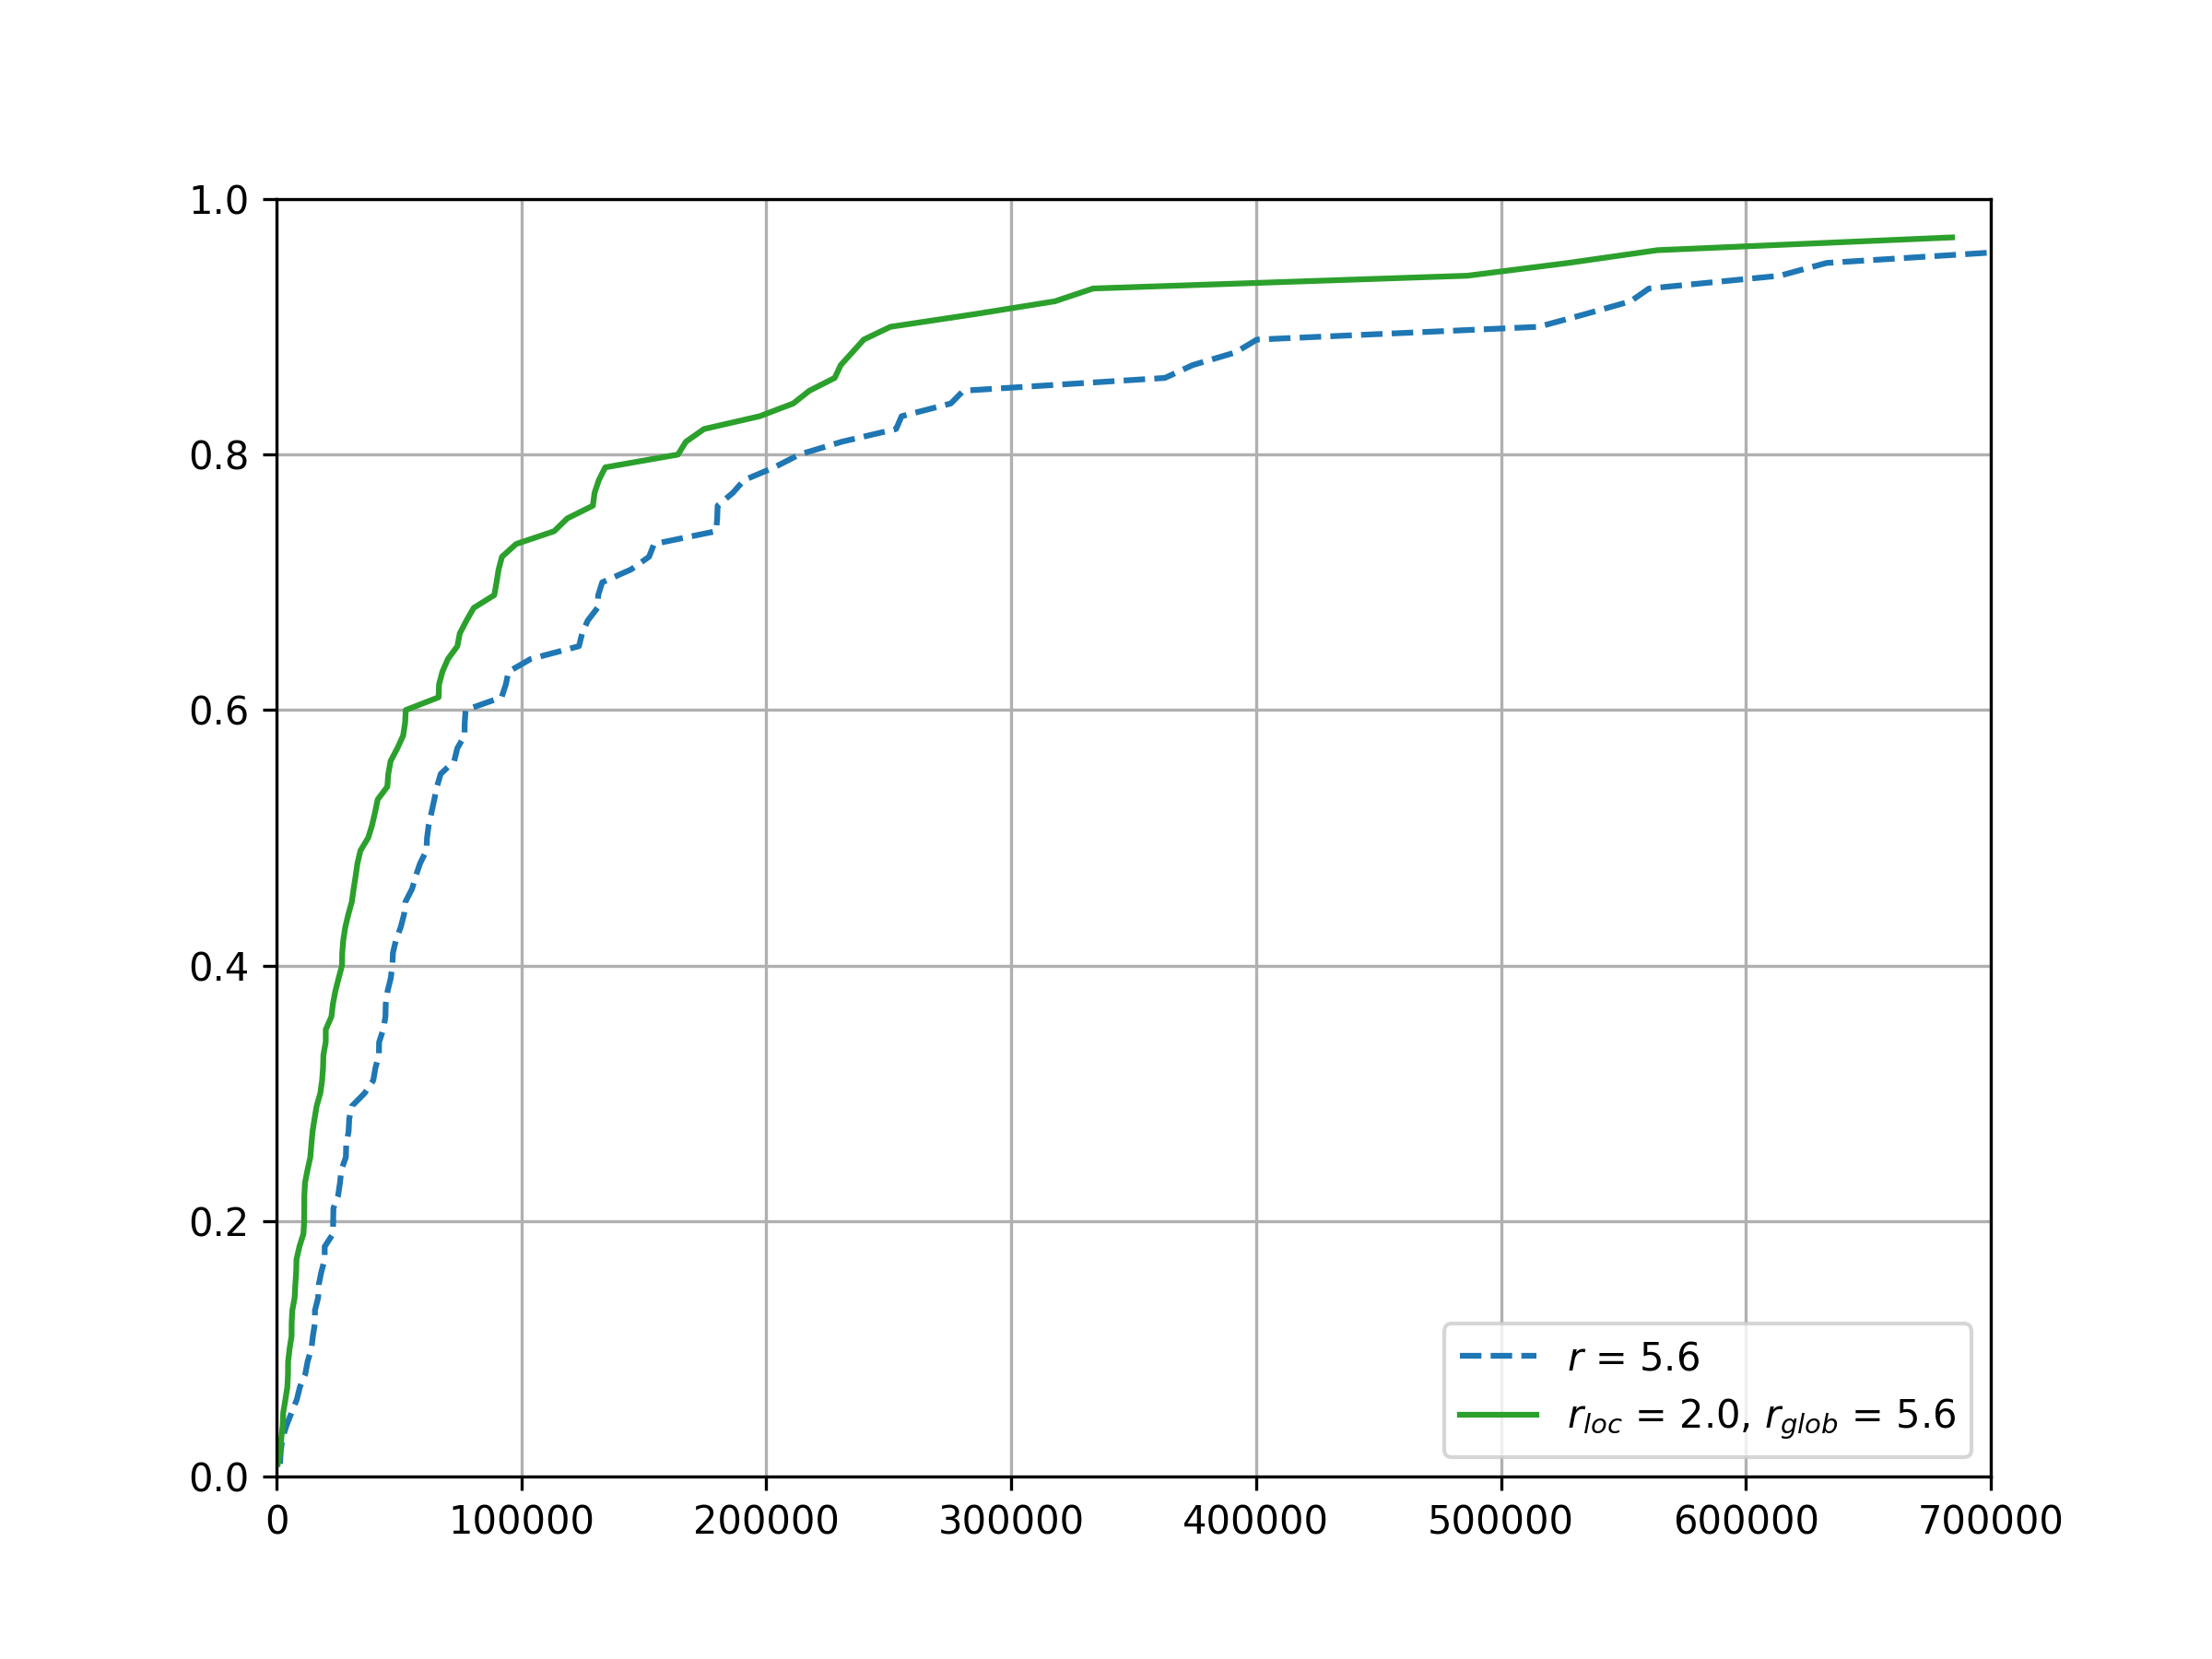
\includegraphics[width=1.0\linewidth]{Operating_characteristic_gklsh_5.png} \\ (b)}
\end{minipage}
\caption{Operational characteristics for GKLS Simple (a) and Hard (b) classes, $N=5$.}
\label{oper5}
\end{figure}

The lower curves in Fig. \ref{oper4} and \ref{oper5} feature GSA whereas the upper ones --- GSA-DL. Such positions of the curves show the algorithm with two estimates of the Lipschitz constant provides much faster solving of the problem series in average that the algorithm using single estimate of the constant.

% ---- Bibliography ----
%
% BibTeX users should specify bibliography style 'splncs04'.
% References will then be sorted and formatted in the correct style.

\bibliographystyle{splncs04}
\bibliography{bibliography}

%\begin{thebibliography}{8}
%\end{thebibliography}
\end{document}
